\documentclass[aspectratio=169]{beamer}

% Theme and Color Scheme
\usetheme{Madrid}
\usecolortheme{beaver}

% Packages
\usepackage[utf8]{inputenc}
\usepackage{graphicx}
\usepackage{tikz}
\usetikzlibrary{shapes, arrows, positioning}
\usepackage{fontawesome5}
\usepackage{xcolor}
\usepackage{amsmath}
\usepackage{array}
\usepackage{textcomp} % For additional text symbols

% Custom Colors
\definecolor{myNewColorA}{RGB}{206,008,20}
\definecolor{myNewColorB}{RGB}{26,168,217}
\definecolor{myNewColorC}{RGB}{245, 233, 85}
\definecolor{darkblue}{RGB}{0,51,102}
\definecolor{lightblue}{RGB}{173,216,230}

\setbeamercolor*{palette primary}{bg=myNewColorC}
\setbeamercolor*{palette secondary}{bg=myNewColorB, fg=white}
\setbeamercolor*{palette tertiary}{bg=myNewColorA, fg=white}
\setbeamercolor*{titlelike}{fg=myNewColorA}
\setbeamercolor*{title}{bg=myNewColorA, fg=white}
\setbeamercolor*{item}{fg=myNewColorA}
\setbeamercolor*{caption name}{fg=myNewColorA}
\usefonttheme{professionalfonts}
\usepackage{natbib}
\usepackage{hyperref}

% Title Information
% \titlegraphic{
\includegraphics[height=1.5cm]{UNESWA_logo.png}} % Commented out if file doesn't exist

\setbeamerfont{title}{size=\large}
\setbeamerfont{subtitle}{size=\small}
\setbeamerfont{author}{size=\small}
\setbeamerfont{date}{size=\small}
\setbeamerfont{institute}{size=\small}

\title[University of Eswatini]{Introduction to Computer Science}
\subtitle{CSC111 - Unit 8: Algorithm, Flowchart and Pseudo-code}
\author[J.S.D]{Mr. Johnson Dlamini}
\institute[jsdlamini@uniswa.sz]{The University of Eswatini}
\date{\today}

\AtBeginSection[]{
  \begin{frame}
  \vfill
  \centering
  \begin{beamercolorbox}[sep=8pt,center,shadow=true,rounded=true]{title}
    \usebeamerfont{title}\insertsectionhead\par%
  \end{beamercolorbox}
  \vfill
  \end{frame}
}

\begin{document}

% Title Slide
\frame{\titlepage}

% Table of Contents
\begin{frame}{Outline}
    \tableofcontents
\end{frame}

% Section 1: Introduction
\section{Introduction}

\begin{frame}{Unit Overview}
    
            \textbf{What we'll explore:}
            \begin{itemize}
                \item Algorithms and their characteristics
                \item Flowcharts and symbols
                \item Pseudo-code development
                \item Program development steps
                \item Structured programming
                \item Generations of programming languages
            \end{itemize}
 
    
    \vspace{0.5cm}
    \begin{alertblock}{Learning Focus}
        Understanding problem-solving methods using algorithms, flowcharts, and pseudo-code for effective programming.
    \end{alertblock}
\end{frame}

\begin{frame}{Learning Outcomes}
    \textbf{After studying this unit, you should be able to:}
    \begin{enumerate}
        \item Define Algorithm and list its characteristics
        \item Describe notations used in algorithm
        \item Define Flowchart and explain its symbols
        \item List and explain program development steps
        \item Describe structured programming
        \item Define Pseudo-code with real-life examples
        \item Explain generations of programming languages
    \end{enumerate}
    
    \vspace{0.3cm}
    \begin{exampleblock}{Key Concepts}
        We'll examine how to represent solutions to problems efficiently using various tools before actual coding.
    \end{exampleblock}
\end{frame}

% Section 2: Algorithm
\section{Algorithm}

\begin{frame}{What is an Algorithm?}
    \begin{definition}
        An \textbf{algorithm} is a step by step or sequential order of solving a problem or to accomplish a task.
    \end{definition}
    
    \vspace{0.3cm}
    \textbf{Key Properties:}
    \begin{itemize}
        \item Best way to represent problem solutions
        \item Simple and efficient representation
        \item Programming language independent
        \item Can be implemented in any programming language
    \end{itemize}
    
    \vspace{0.2cm}
    \begin{exampleblock}{Universal Tool}
        If we have an algorithm for a specific problem, we can implement it in any programming language.
    \end{exampleblock}
\end{frame}

\begin{frame}{Characteristics of an Algorithm}
    \textbf{Seven Essential Features:}
    
    \begin{enumerate}
        \item   Must have a \textbf{beginning} and an \textbf{end}
        \item  Must be simple/clear for \textbf{easy understanding}
        \item  Must have an \textbf{input}
        \item  Must have a \textbf{unique name}
        \item  Must have an \textbf{end result} (desired output)
        \item  Must be \textbf{efficient and effective}
        \item   Must be \textbf{properly planned}
    \end{enumerate}
    
    \vspace{0.5cm}
    \begin{alertblock}{Completeness}
        A good algorithm must be complete - from start to finish with clear inputs and outputs.
    \end{alertblock}
\end{frame}

\begin{frame}{Notations Used in Algorithm}
    \textbf{Two Main Operator Types:}
    
    \begin{columns}
        \begin{column}{0.48\textwidth}
            \begin{block}{\faIcon{calculator} Arithmetic Operators}
                \begin{itemize}
                    \item + (addition)
                    \item - (subtraction)
                    \item * (multiplication)
                    \item \^{} (exponentiation)
                    \item / (Division)
                \end{itemize}
            \end{block}
        \end{column}
        \begin{column}{0.48\textwidth}
            \begin{block}{\faIcon{balance-scale} Relational Operators}
                \begin{itemize}
                    \item $<$ (Less than)
                    \item $>$ (greater than)
                    \item $\neq$ (not equal to)
                    \item $>=$ (greater than or equal to)
                    \item $<=$ (less than or equal to)
                \end{itemize}
            \end{block}
        \end{column}
    \end{columns}
\end{frame}

\begin{frame}{Algorithm Writing Approaches}
    \textbf{Three Problem Perspectives:}
    
    \begin{enumerate}
        \item \textbf{Non-formula Approach}
        \begin{itemize}
            \item No mathematical formulas
            \item Uses logical operators
            \item \textbf{Example}: Directions to school
        \end{itemize}
        
        \item \textbf{Formula Approach}
        \begin{itemize}
            \item Uses mathematical formulas
            \item Arithmetic operators
            \item \textbf{Example}: Area calculations
        \end{itemize}
        
        \item \textbf{Logical Approach}
        \begin{itemize}
            \item Decision-based problems
            \item Conditional statements
            \item \textbf{Example}: Admission eligibility
        \end{itemize}
    \end{enumerate}
\end{frame}

\begin{frame}{Example 1: Non-formula Approach}
    \textbf{Write an algorithm on how to get to school from home}
    
    \begin{exampleblock}{Solution}
        \begin{enumerate}
            \item Step 1: Start
            \item Step 2: Walk to the Bus Rank
            \item Step 3: Take a Kombi
            \item Step 4: Enter the School gate
            \item Step 5: Stop
        \end{enumerate}
    \end{exampleblock}
    
    \vspace{0.3cm}
    \begin{alertblock}{Note}
        This approach doesn't use mathematical formulas - it's purely sequential instructions.
    \end{alertblock}
\end{frame}

\begin{frame}{Example 2: Formula Approach}
    \textbf{Write an algorithm to sum three numbers}
    
    \begin{exampleblock}{Solution} 
            \textbf{Step 1}: Start \\
            \textbf{Step 2}: Input A, B, C  \\
            \textbf{Step 3}: Process D = A + B + C  \\
            \textbf{Step 4}: Print D  \\
            \textbf{Step 5}: Stop 
        
    \end{exampleblock}
    
    \vspace{0.3cm}
    \begin{block}{Variable Types}
        \begin{itemize}
            \item Input variables: A, B, C (right side)
            \item Output variable: D (left side)
        \end{itemize}
    \end{block}
\end{frame}

\begin{frame}{Example 3: Complex Formula Approach}
    \textbf{Write an algorithm to solve quadratic equation}
    
    \begin{exampleblock}{Solution} 
   
            \textbf{Step 1}: Start \\
            \textbf{Step 2}: Input a, b, c \\
            \textbf{Step 3}: Process: \\
                
            \     \   \     \ \textbf{Step 3.1}: $x1 = \frac{-b +  \sqrt{(b² - 4ac)}}{2a} $ \\
            \     \   \     \ \textbf{Step 3.2}: $x2 = \frac{-b -  \sqrt{(b² - 4ac)}}{2a} $
               
            \textbf{Step 4}: Print x1, x2  \\
            \textbf{Step 5}:Stop 
            
   
    


            
    \end{exampleblock}
\end{frame}

\begin{frame}{Example 4: Logical Approach}
    \textbf{Write an algorithm for university admission eligibility}
    
    \begin{exampleblock}{Solution}
         
             \textbf{Step 1}: Start \\
            \textbf{Step 2}: Input credit  \\
             \textbf{Step 3}: If credit $>= 5$ then \\
             \textbf{Step 4}: \ \  \ \ Print "Quality to be considered for admission"  \\
            \textbf{Step 5}: Else  \\
             \textbf{Step 6}: \ \  \ \ Print "Not qualify to be considered for admission"  \\
             \textbf{Step 7}: Stop
       
    \end{exampleblock}
    
    \vspace{0.3cm}
    \begin{alertblock}{Decision Making}
        This uses logical operators to make decisions based on input conditions.
    \end{alertblock}
\end{frame}

\begin{frame}{Activity 1: Practice Problems}
    \textbf{Try these algorithm problems:}
    
    \begin{enumerate}
        \item Write an algorithm to find the average of five numbers
        \item Write an algorithm to calculate the circumference of a circle
    \end{enumerate}
    
    \vspace{0.5cm}
    \begin{block}{Hint}
        Remember the characteristics: Input, Process, Output, and proper start/stop.
    \end{block}
\end{frame}

% Section 3: Flowchart
\section{Flowchart}

\begin{frame}{What is a Flowchart?}
    \begin{definition}
        A \textbf{flowchart} is a graphical representation in which symbols are used to represent operations, data, flow, logic, equipment and so on.
    \end{definition}
    
    \vspace{0.3cm}
    \textbf{Types of Flowcharts:}
    \begin{itemize}
        \item \textbf{Program flowchart} - illustrates program structure and sequence
        \item \textbf{System flowchart} - illustrates information system components and flows
        \item \textbf{Procedure flowchart} - illustrates procedural steps
    \end{itemize}
\end{frame}

\begin{frame}{Flowchart Symbols}
    \textbf{Standard ANSI Symbols:}
    
    \begin{columns}
        \begin{column}{0.3\textwidth}
            \centering
            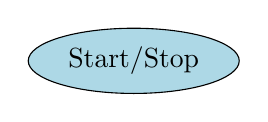
\begin{tikzpicture}
                \node[ellipse, draw, fill=lightblue, minimum width=1.5cm, minimum height=0.8cm] {Start/Stop};
            \end{tikzpicture}
            \\Start/Stop
        \end{column}
        \begin{column}{0.3\textwidth}
            \centering
            \begin{tikzpicture}
                \node[parallelogram, draw, fill=myNewColorC, minimum width=1.5cm, minimum height=0.8cm] {I/O};
            \end{tikzpicture}
            \\Input/Output
        \end{column}
        \begin{column}{0.3\textwidth}
            \centering
            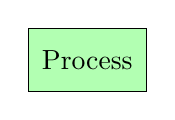
\begin{tikzpicture}
                \node[rectangle, draw, fill=green!30, minimum width=1.5cm, minimum height=0.8cm] {Process};
            \end{tikzpicture}
            \\Process
        \end{column}
    \end{columns}
    
    \vspace{0.5cm}
    \begin{columns}
        \begin{column}{0.3\textwidth}
            \centering
            
\begin{tikzpicture}
                \node[diamond, draw, fill=orange!30, minimum width=1.5cm, minimum height=0.8cm] {Decision};
            \end{tikzpicture}
            \\Decision
        \end{column}
        \begin{column}{0.3\textwidth}
            \centering
            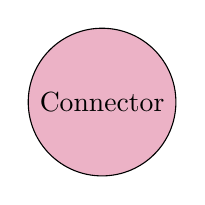
\begin{tikzpicture}
                \node[circle, draw, fill=purple!30, minimum width=1cm] {Connector};
            \end{tikzpicture}
            \\Connector
        \end{column}
        \begin{column}{0.3\textwidth}
            \centering
            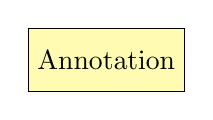
\begin{tikzpicture}
                \node[rectangle, draw, fill=yellow!30, minimum width=1.5cm, minimum height=0.8cm] {Annotation};
            \end{tikzpicture}
            \\Annotation
        \end{column}
    \end{columns}
\end{frame}

\begin{frame}{Flowchart Example}
    \textbf{Draw a flowchart to calculate cylinder volume and surface area}
    
    \centering
    \begin{tikzpicture}[
        node distance=1.2cm,
        startstop/.style={ellipse, draw, fill=lightblue, text width=2.5cm, align=center, minimum height=0.8cm},
        io/.style={parallelogram, draw, fill=myNewColorC, text width=2.5cm, align=center, minimum height=0.8cm},
        process/.style={rectangle, draw, fill=green!30, text width=4cm, align=center, minimum height=0.8cm},
        arrow/.style={->, >=stealth}
    ]
        \node[startstop] (start) {Start};
        \node[io, below of=start] (input) {Input π, R, H};
        \node[process, below of=input] (volume) {$V = \pi * R² * H$};
        \node[process, below of=volume] (area) {$SA = 2 * \pi * R * H$};
        \node[io, below of=area] (output) {Output V, SA};
        \node[startstop, below of=output] (stop) {Stop};
        
        \draw[arrow] (start) -- (input);
        \draw[arrow] (input) -- (volume);
        \draw[arrow] (volume) -- (area);
        \draw[arrow] (area) -- (output);
        \draw[arrow] (output) -- (stop);
    \end{tikzpicture}
\end{frame}

\begin{frame}{Activity 2: Flowchart Practice}
    \textbf{Create flowcharts for:}
    
    \begin{enumerate}
        \item Calculate the area and perimeter of a rectangle
        \item Determine if a student sat for examination in a course or not
    \end{enumerate}
    
    \vspace{0.5cm}
    \begin{block}{Remember}
        Use proper symbols and ensure logical flow from start to finish.
    \end{block}
\end{frame}

% Section 4: Program Development
\section{Program Development}

\begin{frame}{Steps in Program Development: \textbf{Five Key Stages:}} 

    \begin{columns}
        \begin{column}{0.5\textwidth} 
    \begin{enumerate}
    
        \item \textbf{Problem Definition}
        \begin{itemize}
            \item Clarify programming needs
            \item Understand requirements
            \item Define input/output parameters
        \end{itemize}
        
        \item \faIcon{blueprint} \textbf{Solution Design}
        \begin{itemize}
            \item Plan the solution
            \item Work out step-by-step approach
            \item General to detailed design
        \end{itemize}
    \end{enumerate}

    \end{column}


    \begin{column}{0.5\textwidth} 
  
       \begin{enumerate}
        \setcounter{enumi}{2}
        \item \faIcon{code} \textbf{Coding}
        \begin{itemize}
            \item Transcribe solution into programming language
            \item Select appropriate language
            \item Write the actual program
        \end{itemize}
        
        \item \faIcon{bug} \textbf{Program Testing and Correction}
        \begin{itemize}
            \item Test program functionality
            \item Debug errors (bugs)
            \item Use multiple test datasets
            \item Validate results
        \end{itemize}
        
         
    \end{enumerate}
    
    \end{column}
    
    \end{columns}
    \begin{enumerate}
         \setcounter{enumi}{4}
        \item \faIcon{file-alt} \textbf{Documentation}
        \begin{itemize}
            \item Describe problem and solution
            \item Document input/output requirements
            \item User and system documentation
        \end{itemize}
    \end{enumerate}
    
\end{frame}
 

\begin{frame}{Structured Programming}
    \begin{definition}
        \textbf{Structured programming} is a design approach that takes a top-down approach, breaking programs into modular forms using standard logic called CONTROL STRUCTURES.
    \end{definition} 
    
    \textbf{Key Principles:}
    \begin{itemize}
        \item Top-down design approach
        \item Modular program structure
        \item Standard control structures
        \item Clear and correct descriptions
        \item Efficient and organized code
    \end{itemize}
    
    % \vspace{0.2cm}
    \begin{exampleblock}{Design Process}
        \begin{enumerate}
            \item Determine program logic (top-down)
            \item Design in detail (pseudo-code/flowchart)
            \item Test with structured walkthrough
        \end{enumerate}
    \end{exampleblock}
\end{frame}

% Section 5: Pseudo-code
\section{Pseudo-code}

\begin{frame}{What is Pseudo-code?}
    \begin{definition}
        \textbf{Pseudo-code} is a tool for designing a program in narrative form using English-like statements to describe the logic and processing flow.
    \end{definition}
    
    \vspace{0.3cm}
    \textbf{Key Features:}
    \begin{itemize}
        \item English-like statements
        \item Programming language independent
        \item Describes algorithms without syntax
        \item Uses control structure terms (IF, THEN, ELSE)
        \item Follows structured programming rules
    \end{itemize}
    
    \vspace{0.2cm}
    \begin{alertblock}{Advantage}
        Pseudo-code allows algorithm description without knowing specific programming language syntax.
    \end{alertblock}
\end{frame}

\begin{frame}{Pseudo-code Example}
    \textbf{Solve quadratic equation using pseudo-code}
    
    \begin{exampleblock}{Solution}
        \begin{itemize}
            \item READ a, b, c
            \item X1 = -b plus square root of (b² - 4ac) dividing all through by 2 times a
            \item X2 = -b minus square root of (b² - 4ac) dividing all through by 2 times a
            \item Result X1, X2
        \end{itemize}
    \end{exampleblock}
    
    \vspace{0.3cm}
    \begin{block}{Natural Language}
        Pseudo-code uses natural language to describe computational steps clearly and understandably.
    \end{block}
\end{frame}

% Section 6: Programming Language Generations
\section{Programming Language Generations}

\begin{frame}{First Generation Languages}
    \begin{definition}
        \textbf{First Generation}: Machine language - the lowest level language representing data as 1s and 0s.
    \end{definition}
    
    \vspace{0.3cm}
    \textbf{Characteristics:}
    \begin{itemize}
        \item Binary digits (1s and 0s)
        \item Machine-dependent
        \item Direct computer representation
        \item Difficult for humans to read/use
        \item Corresponds to computer's electrical states
    \end{itemize}
    
    \begin{exampleblock}{Machine Language Example}
        \texttt{00101111\ \ 01110011}\\
        \texttt{00101111\ \ 00100000}\\
        \texttt{11001111\ \ 00001100}
    \end{exampleblock}
\end{frame}

\begin{frame}{Second Generation Languages}
    \begin{definition}
        \textbf{Second Generation}: Assembly language - low-level language using abbreviations for instructions.
    \end{definition}
    
    \vspace{0.3cm}
    \textbf{Characteristics:}
    \begin{itemize}
        \item Uses abbreviations (e.g., MUL for multiply)
        \item More readable than machine language
        \item Still machine-dependent
        \item Requires assembler
    \end{itemize}
    
    % \begin{exampleblock}{Assembly Language Example}
    %     \texttt{PACK 210(8,13), 02B(4,7)}\\
    %     \texttt{PACK 218(8,13), 02F(4,7)}\\
    %     \texttt{MUO 212(6,13), 21D(3,13)}
    % \end{exampleblock}

     \begin{exampleblock}{Assembly Language Example (x86)}
        \texttt{MOV AX, 5\hspace{1cm} ; Load 5 into AX register}\\
        \texttt{ADD AX, 3\hspace{1cm} ; Add 3 to AX register}\\
        \texttt{MOV BX, AX\hspace{0.9cm} ; Copy AX to BX register}\\
        \texttt{HLT\hspace{1.7cm} ; Halt execution}
    \end{exampleblock}
    
\end{frame}

\begin{frame}{Third Generation Languages}
    \begin{definition}
        \textbf{Third Generation}: High-level languages (HLL) - procedural languages that set forth procedures to follow.
    \end{definition}
    
    \vspace{0.3cm}
    \textbf{Characteristics:}
    \begin{itemize}
        \item Procedural approach
        \item More English-like
        \item Machine-independent
        \item Requires compiler/interpreter
        \item Examples: FORTRAN, PASCAL, C, COBOL, BASIC
    \end{itemize}
    
    \vspace{0.2cm}
    \begin{exampleblock}{Analogy}
        Like preparing EBA: put water on fire, add Garri when boiling, turn with turner - specific procedures must be followed.
    \end{exampleblock}
\end{frame}

\begin{frame}{Fourth Generation Languages}
    \begin{definition}
        \textbf{Fourth Generation}: Very high-level languages - user-oriented languages requiring fewer commands but more computing power.
    \end{definition}
    
    \vspace{0.3cm}
    \textbf{Characteristics:}
    \begin{itemize}
        \item User-oriented
        \item Fewer commands needed
        \item Non-procedural
        \item More computing power required
        \item Higher abstraction level
    \end{itemize}
    
    \vspace{0.2cm}
    \begin{alertblock}{Non-Procedural}
        Unlike 3GL, 4GL focuses on WHAT needs to be done rather than HOW to do it.
    \end{alertblock}
\end{frame}

\begin{frame}{Fifth Generation Languages}
    \begin{definition}
        \textbf{Fifth Generation}: Natural languages - using human language for more natural connection with computers, part of artificial intelligence (A.I).
    \end{definition}
    
    \vspace{0.3cm}
    \textbf{Two Types:}
    \begin{itemize}
        \item \textbf{Ordinary human languages}: English, Chinese, Siswati, German
        \item \textbf{Programming languages}: Using human language for computer interaction
    \end{itemize}
    
    \vspace{0.3cm}
    \textbf{Examples:}
    \begin{itemize}
        \item Prolog
        \item Lisp
        \item Other AI languages
    \end{itemize}
\end{frame}

% Section 7: Activities and Summary
\section{Activities and Summary}

\begin{frame}{Learning Activities}
    \textbf{Practice Exercises:}
    
    \begin{enumerate}
        \item Differentiate between an algorithm and flowchart
        \item Write an algorithm to solve linear equation
        \item Draw a flowchart for calculating simple interest
        \item Which programming language is used in 4th industrial revolution?
        \item Why does the 3rd industrial revolution support the use of 4GL?
        \item Write a pseudocode to find the average of five numbers
        \item What standard of symbols is used in flowchart?
    \end{enumerate}
\end{frame}

\begin{frame}{Unit Summary}
    \textbf{Key Concepts Covered:}
    
    \begin{columns}
        \begin{column}{0.5\textwidth}
            \begin{itemize}
                \item[\faIcon{check-circle}] \textbf{Algorithms}
                \begin{itemize}
                    \item Step-by-step problem solving
                    \item Characteristics and notations
                    \item Formula vs non-formula approaches
                \end{itemize}
                
                \item[\faIcon{check-circle}] \textbf{Flowcharts}
                \begin{itemize}
                    \item Graphical representation
                    \item ANSI standard symbols
                    \item Program and system flowcharts
                \end{itemize}
            \end{itemize}
        \end{column}
        \begin{column}{0.5\textwidth}
            \begin{itemize}
                \item[\faIcon{check-circle}] \textbf{Program Development}
                \begin{itemize}
                    \item Five key stages
                    \item Structured programming
                    \item Documentation importance
                \end{itemize}
                
                \item[\faIcon{check-circle}] \textbf{Language Generations}
                \begin{itemize}
                    \item 1GL to 5GL evolution
                    \item Machine to natural languages
                    \item AI and future directions
                \end{itemize}
            \end{itemize}
        \end{column}
    \end{columns}
    
    \vspace{0.3cm}
    \begin{block}{Foundation for Programming}
        These tools provide the foundation for effective problem-solving and program development in computer science.
    \end{block}
\end{frame}

\begin{frame}{Thank You}
    \begin{center}
        \Huge{\textbf{Questions?}}
        
        \vspace{1cm}
        \Large{\faIcon{comments} Discussion Time}
    \end{center}
\end{frame}

\end{document}